% =====================================================================
%  CareFlow: Clinical Pathway Process Mining  --  Internship Project Report
%  Compile with pdfLaTeX (Overleaf default). Put all images in /images
% =====================================================================
\documentclass[11pt,a4paper]{article}

\usepackage[T1]{fontenc}
\usepackage[utf8]{inputenc}
\usepackage{lmodern}
\usepackage{microtype}
\usepackage[a4paper,top=2.6cm,bottom=2.4cm,left=2.5cm,right=2.5cm,headheight=15pt]{geometry}
\usepackage{xcolor}
\usepackage{graphicx}
\usepackage{float}
\usepackage{booktabs}
\usepackage{tabularx}
\usepackage{array}
\usepackage{colortbl}
\usepackage{enumitem}
\usepackage{titlesec}
\usepackage{fancyhdr}
\usepackage{caption}
\usepackage{listings}
\usepackage{tikz}
\usepackage[most]{tcolorbox}
\usepackage[hidelinks]{hyperref}
\usepackage{setspace}
\usepackage{tocloft}

% ---------- colours ----------
\definecolor{navy}{HTML}{12365C}
\definecolor{teal}{HTML}{1F8A9E}
\definecolor{amber}{HTML}{E8A33D}
\definecolor{alertred}{HTML}{C0392B}
\definecolor{lightbg}{HTML}{EAF1F6}
\definecolor{greytext}{HTML}{5B6B7C}

\hypersetup{colorlinks=true,linkcolor=navy,urlcolor=teal,citecolor=teal}
\setstretch{1.12}
\setlength{\parskip}{0.55em}
\setlength{\parindent}{0pt}
\setlist{itemsep=0.2em,topsep=0.3em}
\setlist[itemize]{label=\textcolor{teal}{\textbullet}}

% ---------- headings ----------
\titleformat{\section}{\sffamily\Large\bfseries\color{navy}}{\thesection}{0.7em}{}[\vspace{-0.4em}\textcolor{teal}{\titlerule[1.2pt]}]
\titleformat{\subsection}{\sffamily\large\bfseries\color{teal}}{\thesubsection}{0.6em}{}
\titlespacing*{\section}{0pt}{1.6em}{0.9em}
\titlespacing*{\subsection}{0pt}{1.1em}{0.4em}

% ---------- captions ----------
\captionsetup{font={small,it,color=greytext},labelfont={bf,color=navy},labelsep=period,skip=6pt}

% ---------- header / footer ----------
\pagestyle{fancy}
\fancyhf{}
\fancyhead[L]{\sffamily\footnotesize\color{greytext}CareFlow: Clinical Pathway Process Mining}
\fancyhead[R]{\sffamily\footnotesize\color{greytext}Infotact Solutions}
\fancyfoot[L]{\sffamily\footnotesize\color{greytext}Data Analytics Internship | Project Report}
\fancyfoot[R]{\sffamily\footnotesize\color{navy}\thepage}
\renewcommand{\headrulewidth}{0.4pt}
\renewcommand{\footrulewidth}{0pt}
\renewcommand{\headrule}{\hbox to\headwidth{\color{teal}\leaders\hrule height \headrulewidth\hfill}}

% ---------- table styling ----------
\newcommand{\tablehead}[1]{\color{white}\sffamily\bfseries #1}
\renewcommand{\arraystretch}{1.25}
\newcolumntype{L}[1]{>{\raggedright\arraybackslash}p{#1}}
\newcolumntype{Y}{>{\raggedright\arraybackslash}X}
\newcolumntype{C}{>{\centering\arraybackslash}X}

% ---------- callout boxes ----------
\newtcolorbox{keybox}[1][]{enhanced,breakable,colback=lightbg,colframe=teal,boxrule=0pt,
  leftrule=3pt,arc=2pt,left=10pt,right=10pt,top=7pt,bottom=7pt,fonttitle=\sffamily\bfseries,#1}
\newtcolorbox{warnbox}[1][]{enhanced,breakable,colback=amber!10,colframe=amber,boxrule=0pt,
  leftrule=3pt,arc=2pt,left=10pt,right=10pt,top=7pt,bottom=7pt,fonttitle=\sffamily\bfseries,#1}

% ---------- DAX listing ----------
\lstdefinestyle{dax}{basicstyle=\ttfamily\footnotesize,breaklines=true,columns=fullflexible,
  frame=single,rulecolor=\color{teal!50},backgroundcolor=\color{lightbg},xleftmargin=4pt,xrightmargin=4pt,
  aboveskip=0.6em,belowskip=0.6em,showstringspaces=false,keywordstyle=\color{navy}\bfseries,
  morekeywords={DISTINCTCOUNT,DIVIDE,MEDIAN,PERCENTILE,INC,CALCULATE,COUNTROWS}}

% ---------- KPI card (used in the summary) ----------
\newcommand{\kpi}[2]{%
  \parbox[t]{0.178\textwidth}{\begin{tcolorbox}[enhanced,width=\linewidth,colback=white,colframe=lightbg!70!navy,boxrule=0.6pt,
    leftrule=3pt,arc=2pt,left=4pt,right=2pt,top=4pt,bottom=4pt,halign=left,nobeforeafter]
    {\sffamily\scriptsize\color{greytext}#1}\\[1pt]{\sffamily\bfseries\large\color{navy}#2}
  \end{tcolorbox}}}

\begin{document}

% =====================================================================
%  COVER PAGE
% =====================================================================
\begin{titlepage}
\thispagestyle{empty}
\begin{tikzpicture}[remember picture,overlay]
  % top navy block
  \fill[navy] (current page.north west) rectangle ([yshift=-11.2cm]current page.north east);
  % teal accent stripe
  \fill[teal] ([yshift=-11.2cm]current page.north west) rectangle ([yshift=-11.55cm]current page.north east);
  \fill[amber] ([yshift=-11.55cm]current page.north west) rectangle ([xshift=5cm,yshift=-11.7cm]current page.north west);
  % decorative event-flow motif
  \foreach \x/\y in {13.2/-2.4, 15.0/-3.6, 16.8/-2.4, 18.6/-3.6}{
    \fill[white,opacity=0.14] ([xshift=\x cm,yshift=\y cm]current page.north west) circle (0.28);
  }
  \draw[white,opacity=0.14,line width=1.6pt] ([xshift=13.2cm,yshift=-2.4cm]current page.north west)
    -- ([xshift=15cm,yshift=-3.6cm]current page.north west)
    -- ([xshift=16.8cm,yshift=-2.4cm]current page.north west)
    -- ([xshift=18.6cm,yshift=-3.6cm]current page.north west);
\end{tikzpicture}

\vspace*{1.2cm}
{\color{white}\sffamily\bfseries\large\hspace{0.1cm}INFOTACT SOLUTIONS}\\[0.15cm]
{\color{white!80!navy}\sffamily\hspace{0.1cm}Data Analytics Internship \textbar{} Project Report}

\vspace{2.3cm}
{\color{white}\sffamily\bfseries\fontsize{40}{44}\selectfont\hspace{0.1cm}CareFlow}\\[0.35cm]
{\color{white}\sffamily\fontsize{20}{24}\selectfont\hspace{0.1cm}Clinical Pathway Process Mining}\\[0.5cm]
{\color{white!85!navy}\sffamily\large\hspace{0.1cm}An Emergency Department event-log dashboard built with Power BI}

\vspace{4.6cm}
\begin{tabular}{@{}p{3.9cm}p{10.4cm}@{}}
  \textsf{\textbf{\textcolor{navy}{Assignment reference}}} & ITS/DA/1135\\[5pt]
  \textsf{\textbf{\textcolor{navy}{Team}}} & Team Group No.\ 5\\[5pt]
  \textsf{\textbf{\textcolor{navy}{Prepared by}}} & Gorige Sravani (BI and Dashboard Development)\\[5pt]
  \textsf{\textbf{\textcolor{navy}{Team members}}} & Piyusha Sanjay Patil, Atharv Rajendra Talaskar, Gorige Sravani\\[5pt]
  \textsf{\textbf{\textcolor{navy}{Internship period}}} & 5 October 2026 to 5 November 2026\\[5pt]
  \textsf{\textbf{\textcolor{navy}{Submission}}} & November 2026
\end{tabular}

\vfill
{\footnotesize\color{greytext}\itshape All figures in this report come from a de-identified Emergency Department demonstration extract and describe recorded data only.}
\end{titlepage}

% =====================================================================
%  ABSTRACT + CONTENTS
% =====================================================================
\pagenumbering{roman}
\section*{Abstract}
\addcontentsline{toc}{section}{Abstract}
Hospital administrators usually see a single average Emergency Department (ED) wait time, which hides the sequence of events behind each visit. \textbf{CareFlow} applies process mining to a de-identified ED demonstration extract of \textbf{222 visits} and \textbf{5,328 recorded events}. The team prepared an event log, discovered how the five recorded activities follow each other, measured the time between recorded events, and presented the findings in a four-page interactive Power BI dashboard. The median ED stay is \textbf{5.84 hours}, 28.4\% of visits last longer than eight hours, and a vitals record exists for 92.8\% of visits. Equally important, the report states what the extract \emph{cannot} show: gaps are time between recorded events and not confirmed waiting times, and no bottleneck or clinical outcome can be concluded from this data.

\vspace{0.6em}
\noindent\textbf{Keywords:} process mining, event log, Emergency Department, Power BI, DAX, PM4Py, data quality.

\vspace{0.8em}
\noindent
\kpi{ED visits}{222}\hfill\kpi{Recorded events}{5,328}\hfill\kpi{Median stay}{5.84 h}\hfill\kpi{Visits over 8 h}{28.4\%}\hfill\kpi{With vitals}{92.8\%}

\newpage
\renewcommand{\contentsname}{\sffamily\bfseries\color{navy}Contents}
\tableofcontents
\vspace{1em}
\renewcommand{\listfigurename}{\sffamily\bfseries\color{navy}List of Figures}
\renewcommand{\listtablename}{\sffamily\bfseries\color{navy}List of Tables}
\listoffigures
\vspace{1em}
\listoftables
\newpage
\pagenumbering{arabic}

% =====================================================================
\section{Introduction}
Hospital administrators often see only an average ED wait time, which cannot show the sequence of events a patient goes through. Process mining addresses this by rebuilding the sequence of recorded events for each visit from timestamped event logs.

CareFlow is a project in the Advanced Data Analytics portfolio of Infotact Solutions. Its aim is to turn ED event records into an event log, discover how recorded activities follow each other, and present the findings in an interactive dashboard.

\subsection{Objectives}
\begin{itemize}
  \item Prepare an event log in the \texttt{Case\_ID}, \texttt{Activity\_Name}, \texttt{Timestamp} format.
  \item Discover recorded activity sequences and measure the time between recorded events.
  \item Build an interactive Power BI dashboard with KPI, flow, gap and data-quality views.
  \item State clearly what the data can and cannot show.
\end{itemize}

\subsection{Scope note}
\begin{warnbox}[title=Scope of the available data]
The project brief describes an example in which patients return to Triage after an X-Ray. The data available to the team contains only five recorded activities and does not include Triage, X-Ray, doctor or diagnosis events, so that example could not be tested. This report therefore describes what the available data supports and does not claim bottlenecks or clinical delays.
\end{warnbox}

% =====================================================================
\section{Team and Responsibilities}
The team divided the work into three connected modules. The output of each module is the input of the next (Figure~\ref{fig:pipeline}).

\begin{table}[H]
\centering
\begin{tabularx}{\textwidth}{L{3.6cm}L{4.2cm}Y}
\rowcolor{navy}\tablehead{Member} & \tablehead{Module} & \tablehead{Responsibility}\\
\rowcolor{lightbg}Piyusha Sanjay Patil & Data engineering and preparation & Event-log creation, cleaning, standardisation and validation\\
Atharv Rajendra Talaskar & Process mining and analysis & Process discovery, variants, repeated activities, recorded-gap analysis\\
\rowcolor{lightbg}Gorige Sravani & BI and dashboard development & Power BI dashboard, KPIs, documentation and presentation\\
\end{tabularx}
\caption{Team roles.}
\end{table}

\begin{figure}[H]
\centering
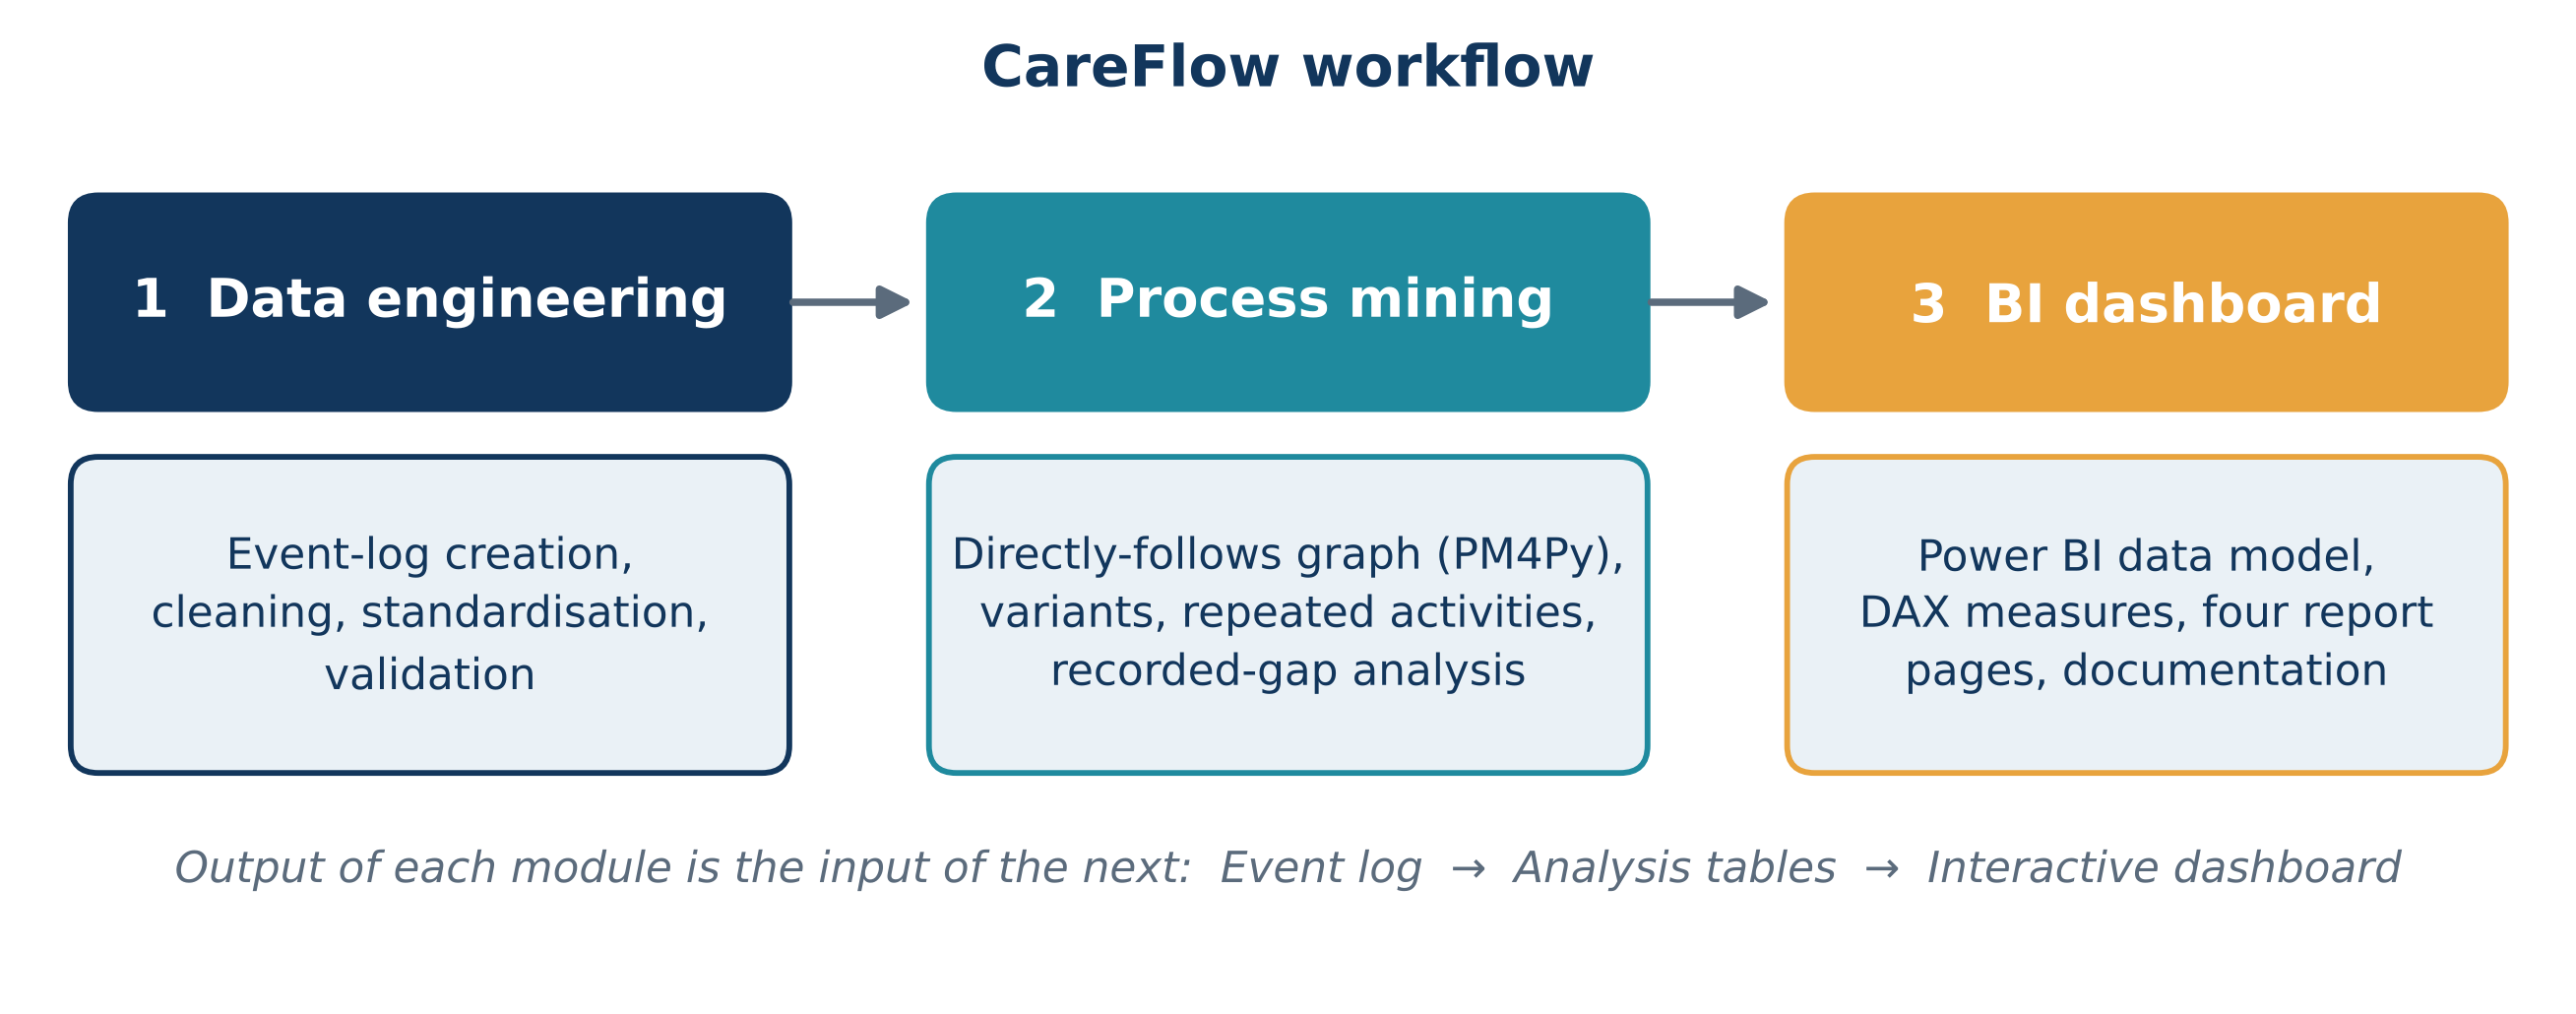
\includegraphics[width=\textwidth]{images/fig_pipeline.png}
\caption{CareFlow workflow: three connected modules from raw records to dashboard.}
\label{fig:pipeline}
\end{figure}

% =====================================================================
\section{Data}
The analysis uses a de-identified ED demonstration extract prepared by the data-engineering module. Each row of the cleaned event log is one recorded event with the columns \texttt{Case\_ID}, \texttt{Activity\_Name}, \texttt{Timestamp}, \texttt{Source\_Table}, \texttt{Source\_Record\_ID} and \texttt{Event\_Type}.

\begin{table}[H]
\centering
\begin{tabularx}{\textwidth}{L{4.2cm}Y}
\rowcolor{navy}\tablehead{Characteristic} & \tablehead{Value}\\
\rowcolor{lightbg}ED visits (cases) & 222\\
Recorded events & 5,328\\
\rowcolor{lightbg}Distinct activities & 5\\
Events per visit & minimum 2, median 21, mean 24.0, maximum 76\\
\rowcolor{lightbg}Activities & ED Arrival, Vitals Recorded, Medication Reconciliation Recorded, Pyxis Medication Record, ED Departure\\
Dates & De-identified (shifted); calendar dates are not analysed\\
\end{tabularx}
\caption{Data overview.}
\end{table}

\begin{keybox}
Triage and diagnosis are not timestamped in the source data and are absent from the event log. Pyxis records show that a medication record exists, not that a medication was given.
\end{keybox}

% =====================================================================
\section{Methodology}
\subsection{Pipeline}
\begin{itemize}
  \item \textbf{Data preparation:} source records were combined into one event log, standardised and validated by the data-engineering module.
  \item \textbf{Process analysis:} a directly-follows graph was discovered with the PM4Py library. Variants, repeated activities, review flags and the time between consecutive recorded events were calculated.
  \item \textbf{Dashboard:} the analysis outputs were loaded into Microsoft Power BI Desktop, related by \texttt{Case\_ID}, and summarised with DAX measures.
\end{itemize}

\subsection{Dashboard data model}
The dashboard uses one central table with one row per visit, related by \texttt{Case\_ID} to the supporting tables (Figure~\ref{fig:model}, Table~\ref{tab:model}).

\begin{figure}[H]
\centering
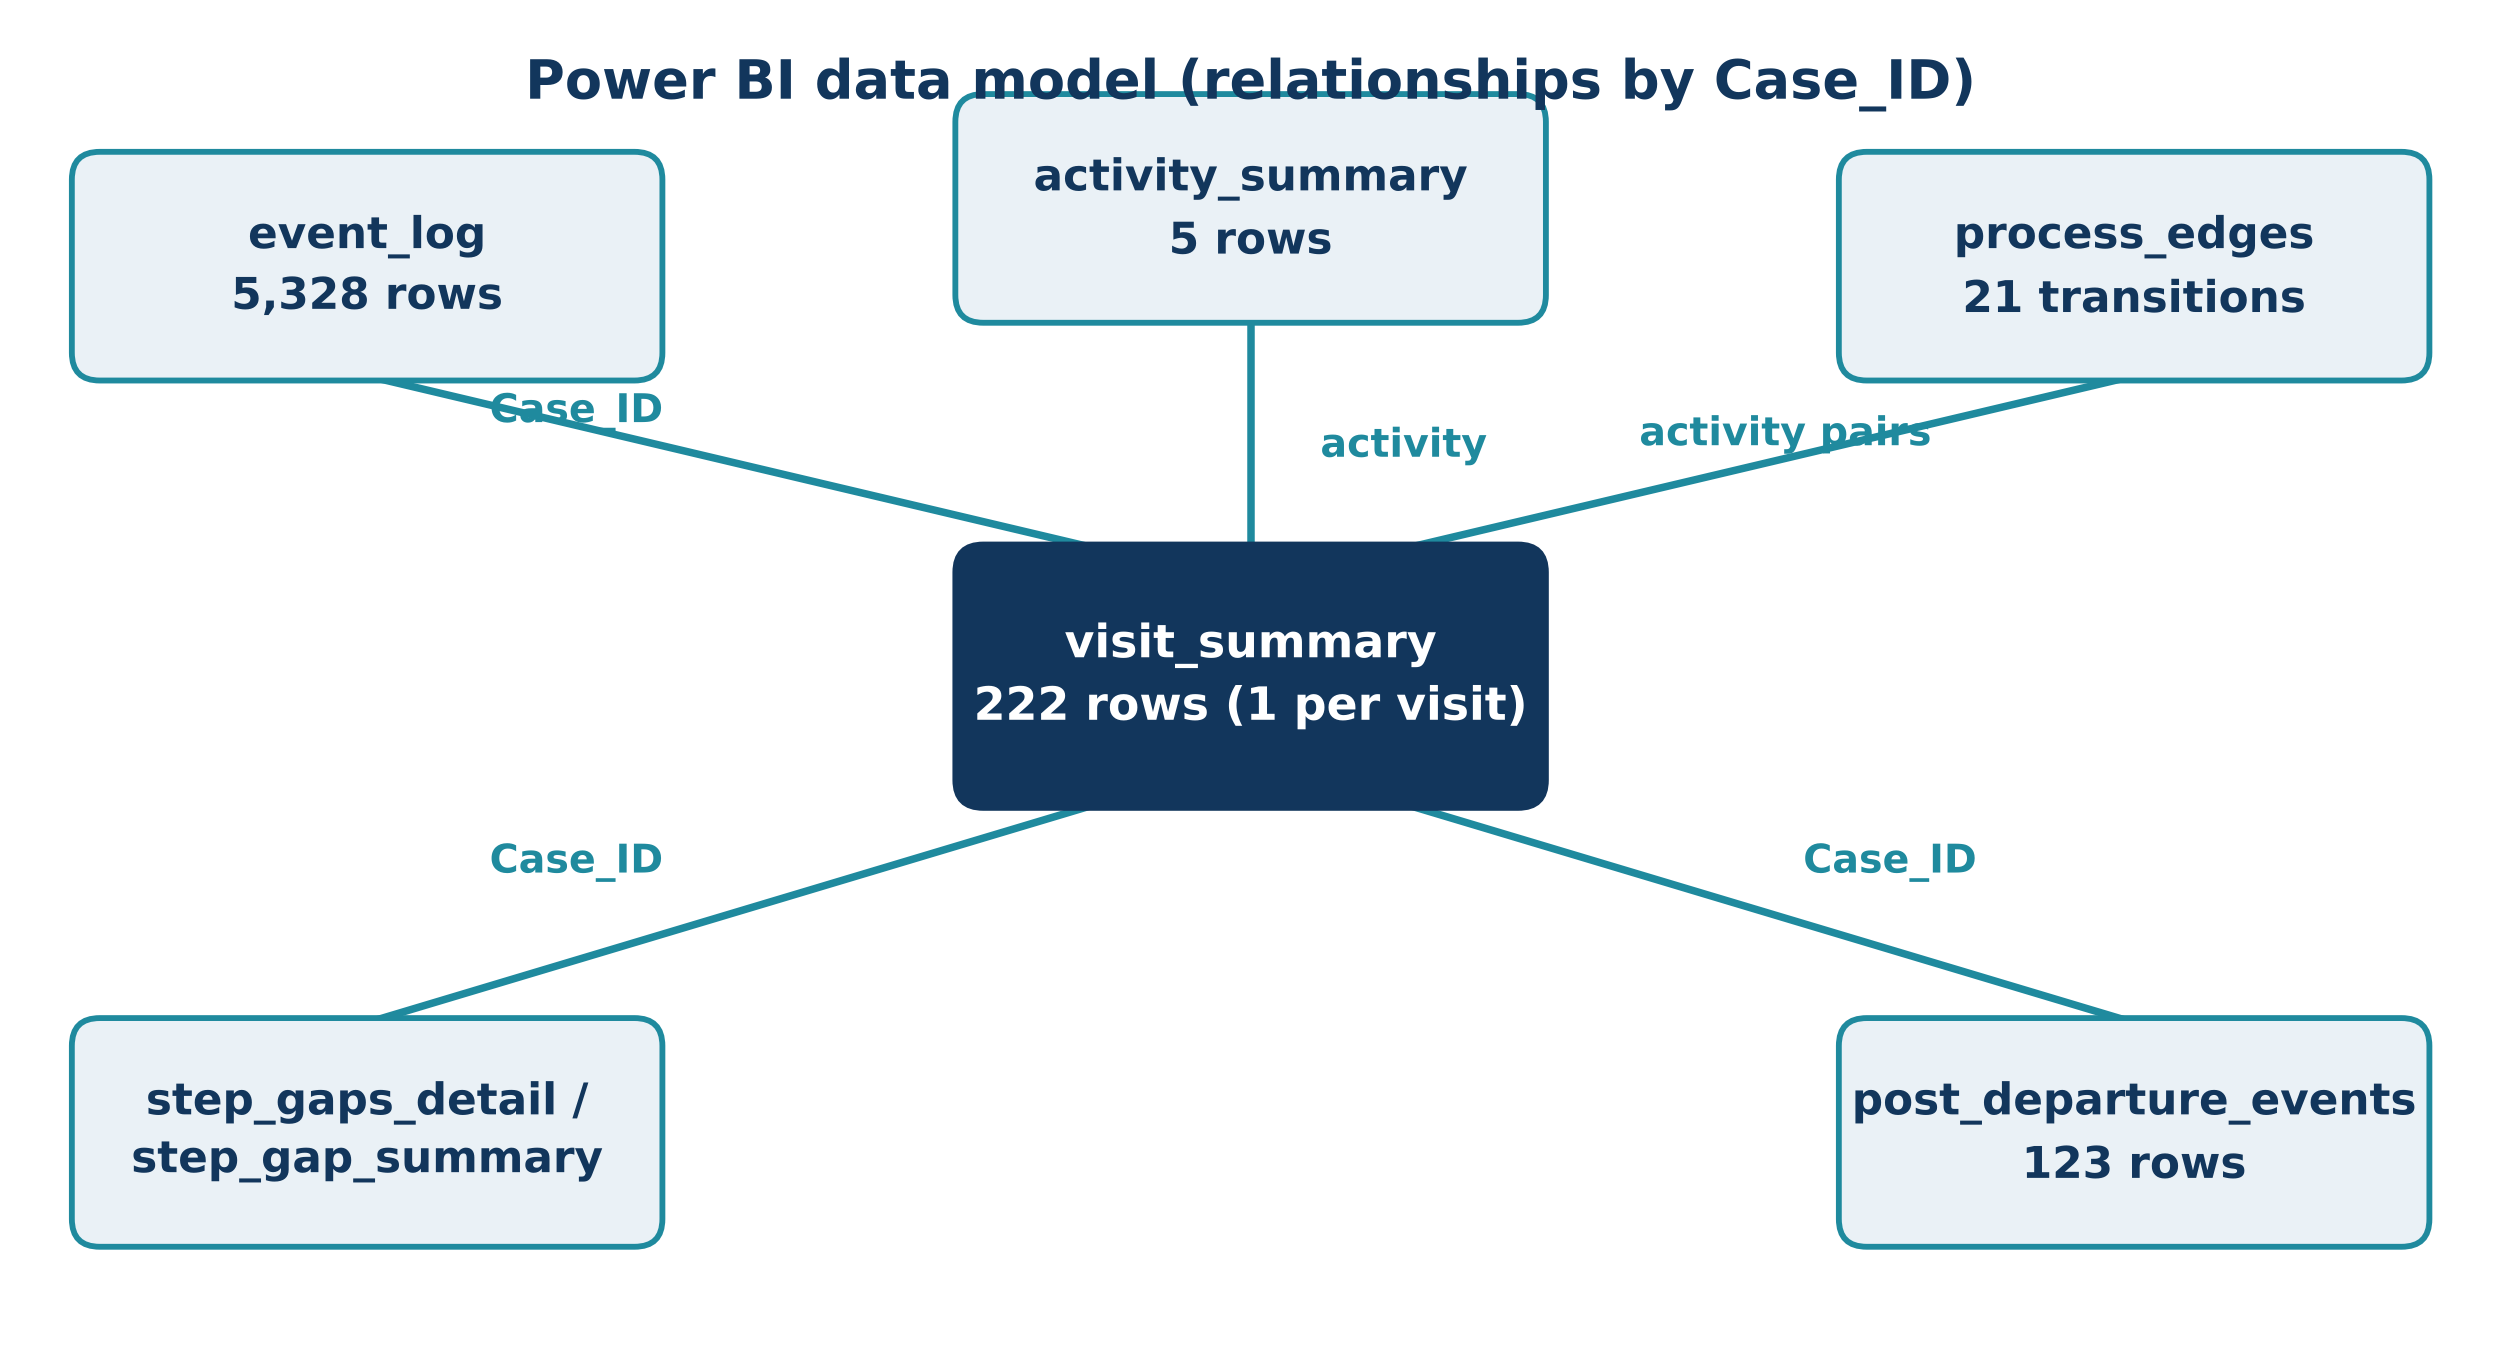
\includegraphics[width=0.95\textwidth]{images/fig_data_model.png}
\caption{Power BI data model.}
\label{fig:model}
\end{figure}

\begin{table}[H]
\centering
\begin{tabularx}{\textwidth}{L{4.6cm}L{3.9cm}Y}
\rowcolor{navy}\tablehead{Table} & \tablehead{One row per} & \tablehead{Used for}\\
\rowcolor{lightbg}\texttt{visit\_summary} & ED visit (222) & KPIs, length of stay, arrival hour and shift, data-quality flags\\
\texttt{event\_log} & Event (5,328) & Event counts per visit\\
\rowcolor{lightbg}\texttt{activity\_summary} & Activity (5) & Share of visits containing each activity\\
\texttt{process\_edges} & Activity pair & Transition matrix\\
\rowcolor{lightbg}\texttt{step\_gap\_summary} / \texttt{step\_gaps\_detail} & Step pair / step & Recorded event gaps\\
\texttt{post\_departure\_events} & Late record (123) & Events recorded after ED Departure\\
\end{tabularx}
\caption{Tables in the Power BI model.}
\label{tab:model}
\end{table}

\subsection{Definitions}
\begin{itemize}
  \item \textbf{Length of stay (LOS):} time from the visit's ED Arrival to its ED Departure.
  \item \textbf{Recorded event gap:} time between two consecutive recorded events of the same visit. It is \emph{not} a confirmed waiting time.
  \item \textbf{Arrival shift:} derived from the arrival hour (Morning 06:00--13:59, Evening 14:00--21:59, Night otherwise).
  \item \textbf{Post-departure event:} a non-departure record with a timestamp later than the visit's ED Departure.
\end{itemize}

% =====================================================================
\section{Dashboard Design}
The dashboard has four pages with a shared layout: a title banner, filters where they apply, KPI cards, visuals and a source footer. Navy and teal are used for ordinary values and red only for data-quality flags, so that colour never suggests poor care.

\begin{table}[H]
\centering
\begin{tabularx}{\textwidth}{L{3.5cm}L{4cm}Y}
\rowcolor{navy}\tablehead{Page} & \tablehead{Purpose} & \tablehead{Main visuals}\\
\rowcolor{lightbg}1. Overview & Volume and length of stay & Five KPI cards, visits by length of stay, arrivals by hour, median stay by shift, longest stays, shift and stay-length slicers\\
2. Activities and flow & What was recorded and in what order & Total events, events per visit, share of visits with vitals, activity share chart, transition matrix\\
\rowcolor{lightbg}3. Recorded event gaps & Time between recorded events & Gap KPIs, median gap by step, gap-size distribution, gap summary by step\\
4. Data quality and limitations & Checks and limits & Four flag cards, post-departure events by activity and by hours, limitations box\\
\end{tabularx}
\caption{Dashboard pages.}
\end{table}

\subsection{Dashboard screenshots}

\begin{figure}[H]
\centering
\fbox{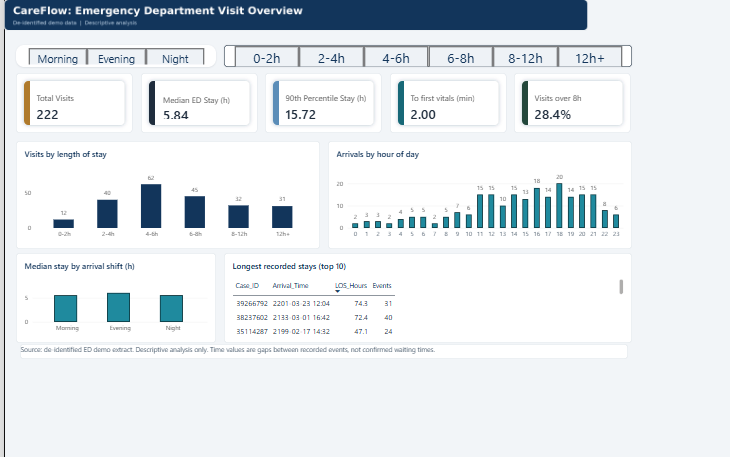
\includegraphics[width=0.96\textwidth]{images/page1_overview.png}}
\caption{Page 1, Overview: volume, length of stay, arrivals by hour and longest recorded stays.}
\label{fig:p1}
\end{figure}

\begin{figure}[H]
\centering
\fbox{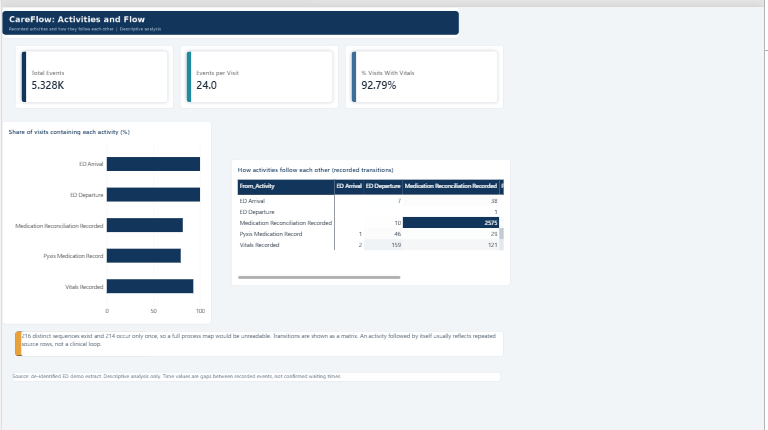
\includegraphics[width=0.96\textwidth]{images/page2_activities_flow.png}}
\caption{Page 2, Activities and flow: activity coverage and the transition matrix.}
\label{fig:p2}
\end{figure}

\begin{figure}[H]
\centering
\fbox{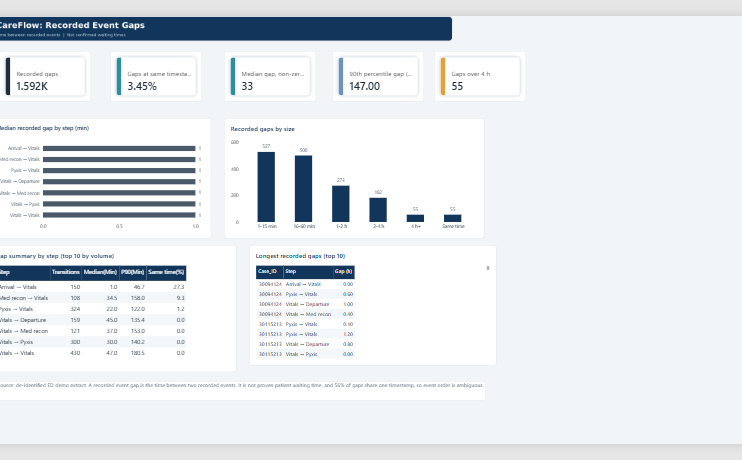
\includegraphics[width=0.96\textwidth]{images/page3_event_gaps.png}}
\caption{Page 3, Recorded event gaps: time between recorded events by step and by size.}
\label{fig:p3}
\end{figure}

\begin{figure}[H]
\centering
\fbox{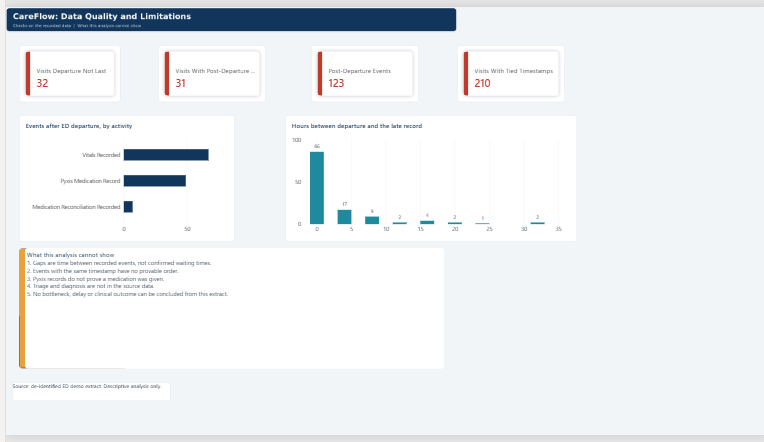
\includegraphics[width=0.96\textwidth]{images/page4_data_quality.png}}
\caption{Page 4, Data quality and limitations: flags, post-departure events and what the analysis cannot show.}
\label{fig:p4}
\end{figure}

% =====================================================================
\section{Results}
All results are descriptive and apply to this extract only.

\subsection{Length of stay and arrivals}

\begin{table}[H]
\centering
\begin{tabularx}{\textwidth}{L{6cm}Y}
\rowcolor{navy}\tablehead{Measure} & \tablehead{Value}\\
\rowcolor{lightbg}Total ED visits & 222\\
Median ED stay & 350.5 minutes (5.84 hours)\\
\rowcolor{lightbg}90th percentile stay & 15.72 hours\\
Visits longer than 8 hours & 63 (28.4\%)\\
\rowcolor{lightbg}Median time from arrival to first vitals record & 2 minutes (206 of 222 visits have a vitals record, 92.8\%)\\
\end{tabularx}
\caption{Key dashboard measures.}
\end{table}

\begin{figure}[H]
\centering
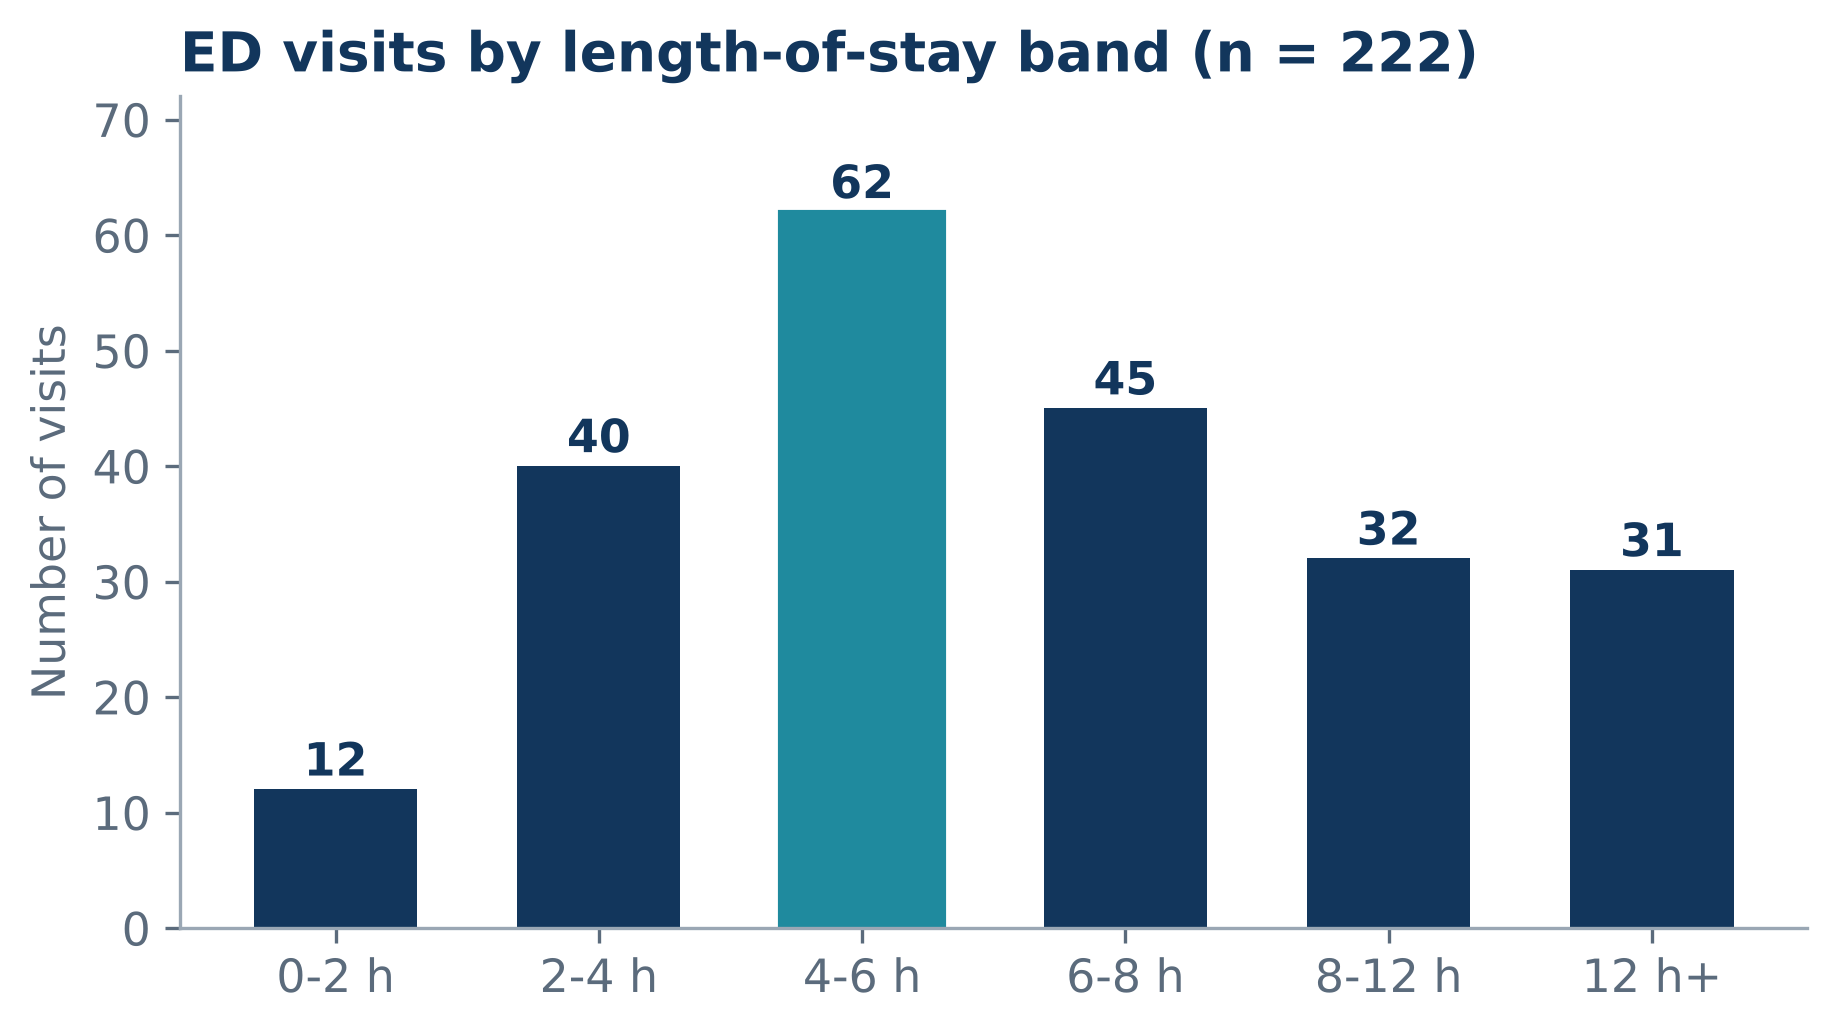
\includegraphics[width=0.82\textwidth]{images/fig_los_bands.png}
\caption{Visits by length-of-stay band (total 222).}
\label{fig:los}
\end{figure}

Most visits lasted between two and eight hours, with the largest group (62 visits) staying four to six hours. Thirty-one visits lasted twelve hours or more. The longest recorded stays were 74.3, 72.4 and 47.1 hours; they are described here as recorded values and are not interpreted as delays.

Arrivals were lowest overnight (two to five visits per hour) and highest in the late afternoon and evening, with a peak of 20 visits at 18:00. Median stay by arrival shift was 5.6 hours (Morning), 6.0 hours (Evening) and 5.6 hours (Night). These differences are small and are described, not explained.

\subsection{Activities and transitions}

\begin{table}[H]
\centering
\begin{tabularx}{\textwidth}{L{6.6cm}CC}
\rowcolor{navy}\tablehead{Activity} & \tablehead{Visits containing it} & \tablehead{Share of visits}\\
\rowcolor{lightbg}ED Arrival & 222 & 100\%\\
ED Departure & 222 & 100\%\\
\rowcolor{lightbg}Vitals Recorded & 206 & 92.8\%\\
Medication Reconciliation Recorded & 181 & 81.5\%\\
\rowcolor{lightbg}Pyxis Medication Record & 176 & 79.3\%\\
\end{tabularx}
\caption{Share of visits containing each activity.}
\end{table}

\begin{figure}[H]
\centering
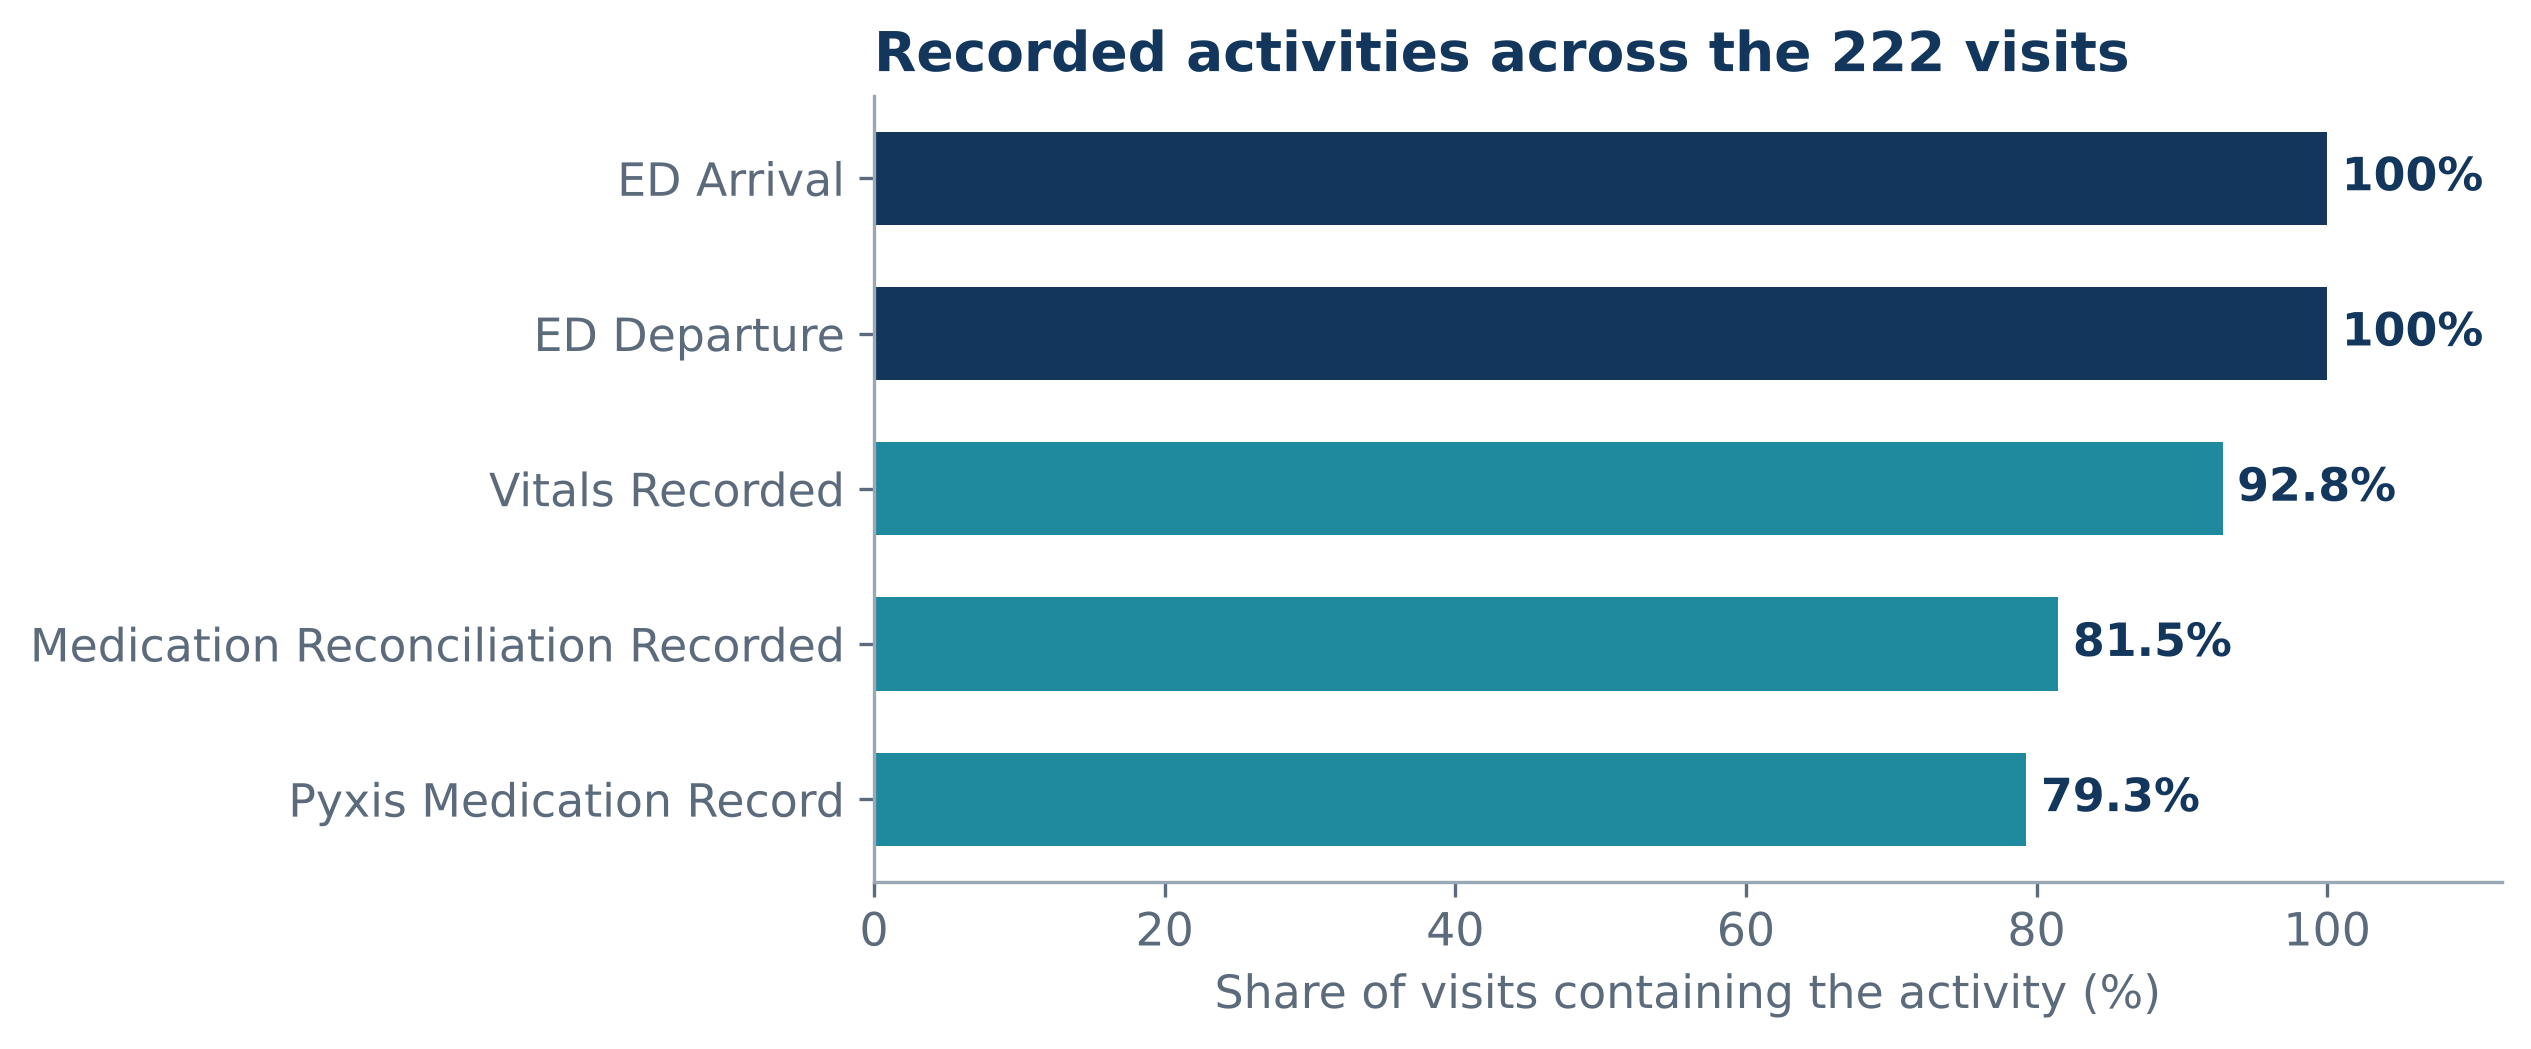
\includegraphics[width=0.82\textwidth]{images/fig_activity_share.png}
\caption{Recorded activities across the 222 visits.}
\end{figure}

There are 216 distinct recorded sequences and 214 of them occur only once, so a full process map would be unreadable. The 21 observed transitions are therefore shown as a matrix (Figure~\ref{fig:p2}). The most frequent transitions are repeats of the same activity, which usually reflect repeated source rows and not a clinical loop.

\begin{table}[H]
\centering
\begin{tabularx}{\textwidth}{YC}
\rowcolor{navy}\tablehead{Transition (from $\rightarrow$ to)} & \tablehead{Recorded transitions}\\
\rowcolor{lightbg}Medication Reconciliation $\rightarrow$ Medication Reconciliation & 2,575\\
Pyxis Medication Record $\rightarrow$ Pyxis Medication Record & 676\\
\rowcolor{lightbg}Vitals Recorded $\rightarrow$ Vitals Recorded & 430\\
Pyxis Medication Record $\rightarrow$ Vitals Recorded & 324\\
\rowcolor{lightbg}Vitals Recorded $\rightarrow$ Pyxis Medication Record & 300\\
Vitals Recorded $\rightarrow$ ED Departure & 159\\
\rowcolor{lightbg}ED Arrival $\rightarrow$ Vitals Recorded & 150\\
\end{tabularx}
\caption{Most frequent recorded transitions.}
\end{table}

\begin{figure}[H]
\centering
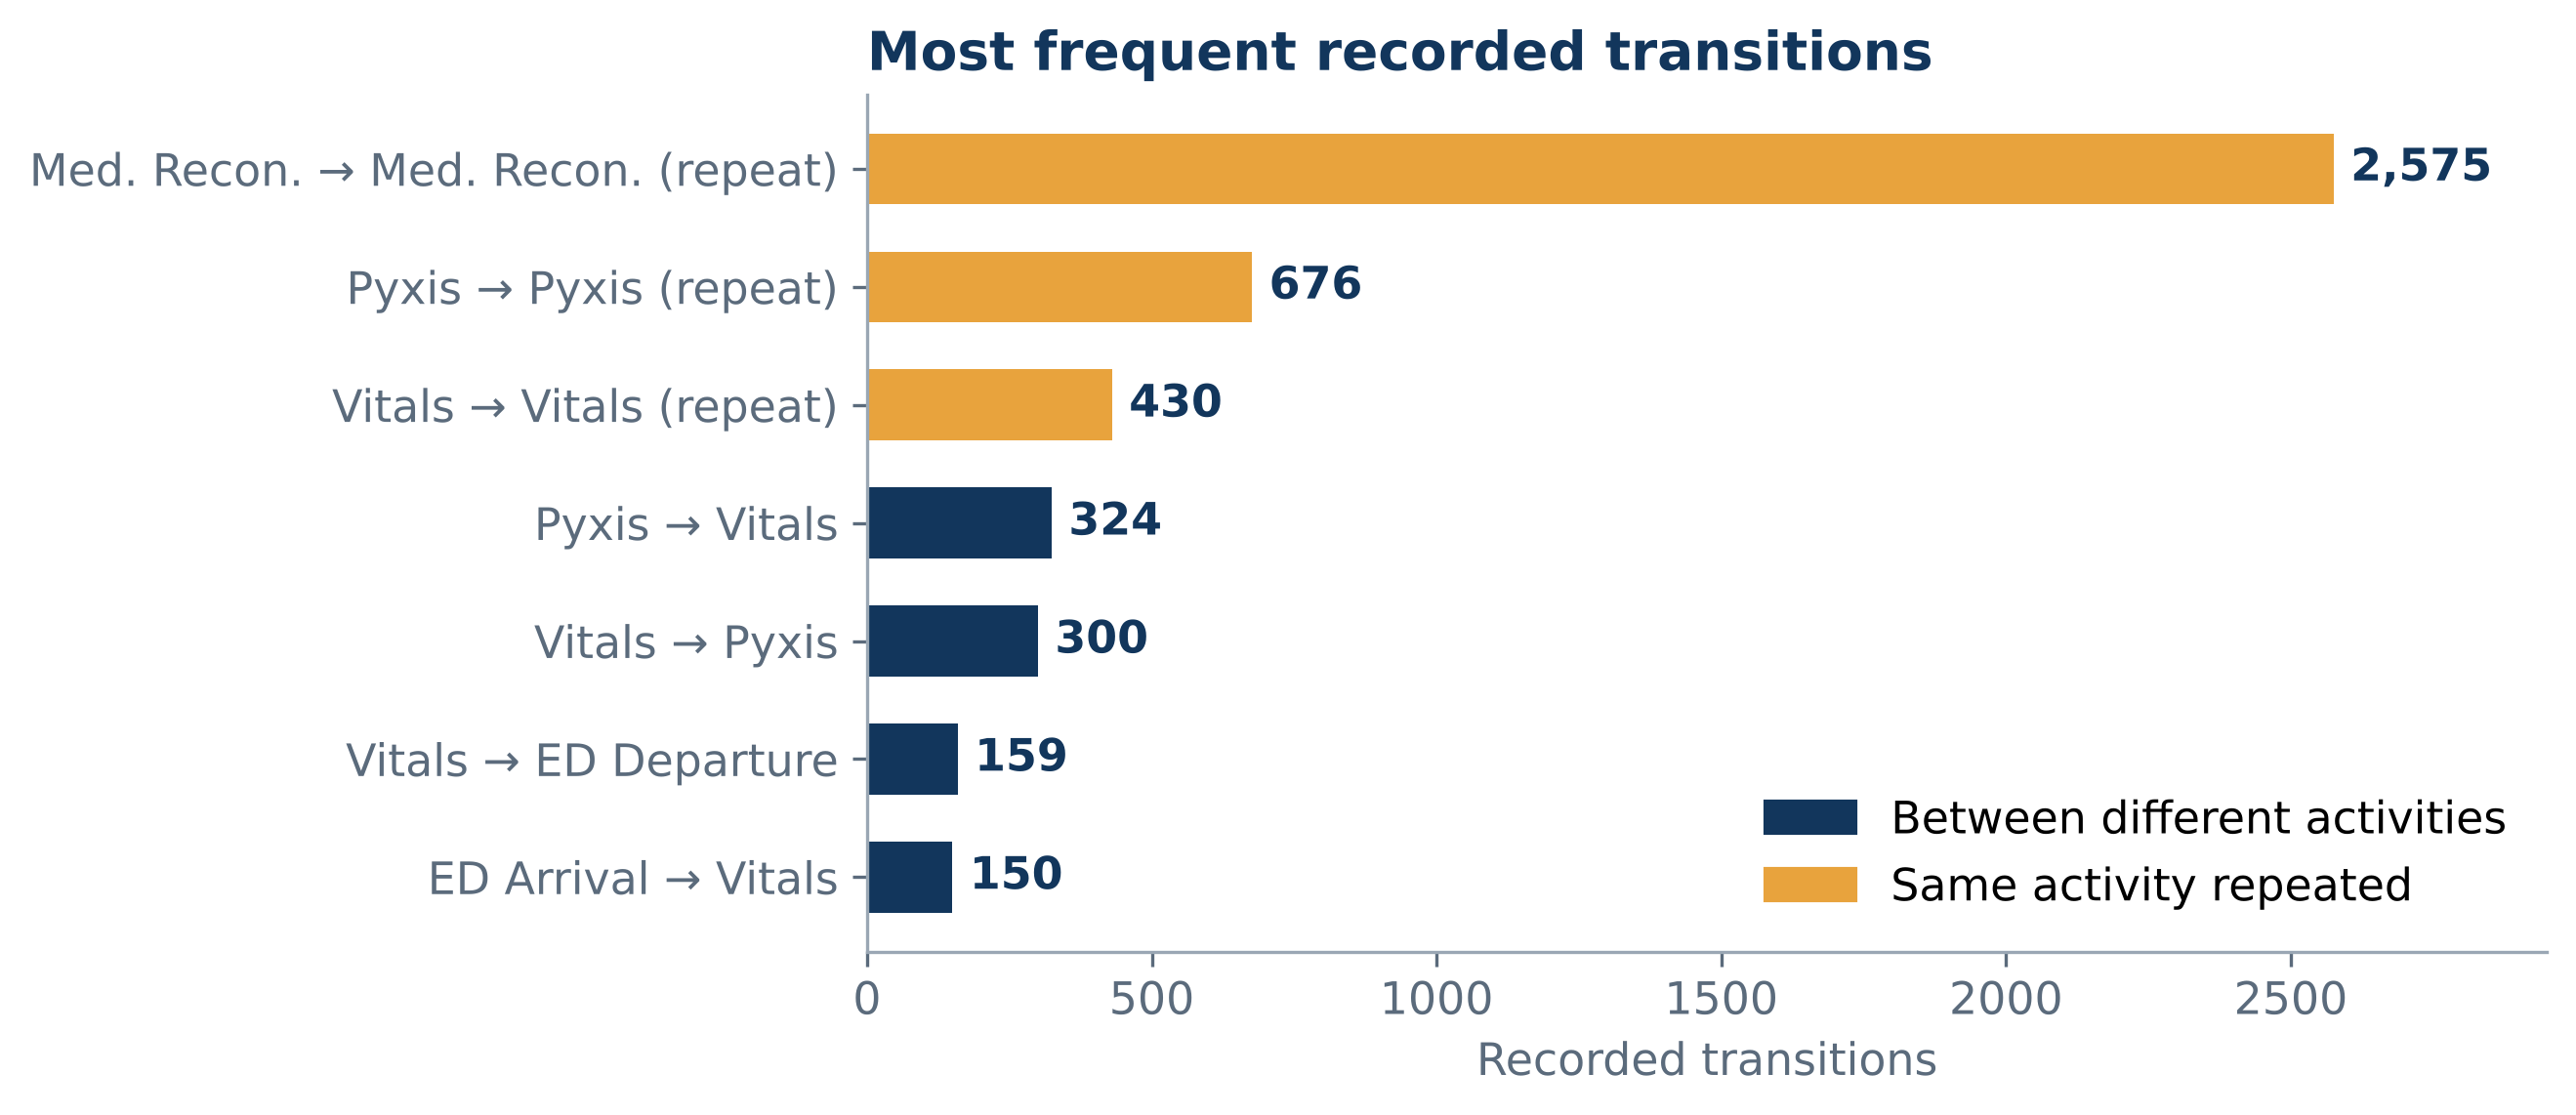
\includegraphics[width=0.88\textwidth]{images/fig_transitions.png}
\caption{Most frequent recorded transitions; amber bars are repeats of the same activity.}
\end{figure}

\subsection{Recorded event gaps}
A recorded event gap is the time between two consecutive recorded events of one visit. Page~3 of the dashboard (Figure~\ref{fig:p3}) summarises them.

\begin{table}[H]
\centering
\begin{tabularx}{\textwidth}{L{7.2cm}Y}
\rowcolor{navy}\tablehead{Measure} & \tablehead{Value}\\
\rowcolor{lightbg}Recorded gaps analysed & 1,592\\
Median gap, excluding zero-length gaps & 33 minutes\\
\rowcolor{lightbg}90th percentile gap & 147 minutes\\
Gaps over 4 hours & 55\\
\end{tabularx}
\caption{Recorded event gap summary (dashboard page 3).}
\end{table}

The gap-size chart groups gaps into same-time, 1--15 minutes, 16--60 minutes, 1--2 hours, 2--4 hours and over 4 hours; most gaps fall in the two shortest minute bands. Because some events share an identical timestamp, the order of those events is not provable. Gaps are time between recorded events and must not be read as patient waiting time.

% =====================================================================
\section{Data Quality and Limitations}

\begin{table}[H]
\centering
\begin{tabularx}{\textwidth}{L{6.3cm}Y}
\rowcolor{navy}\tablehead{Check} & \tablehead{Result}\\
\rowcolor{lightbg}Visits where ED Departure is not the last recorded event & 32\\
Visits with records timestamped after ED Departure & 31 visits, 123 events (Vitals 67, Pyxis 49, Medication Reconciliation 7)\\
\rowcolor{lightbg}Time after departure of those records & median 1.85 hours, maximum 35.3 hours\\
Visits with events sharing an identical timestamp & 210\\
\rowcolor{lightbg}Visits not starting with ED Arrival & 3 (2 start with Vitals, 1 with Pyxis)\\
\end{tabularx}
\caption{Data-quality checks.}
\end{table}

\begin{figure}[H]
\centering
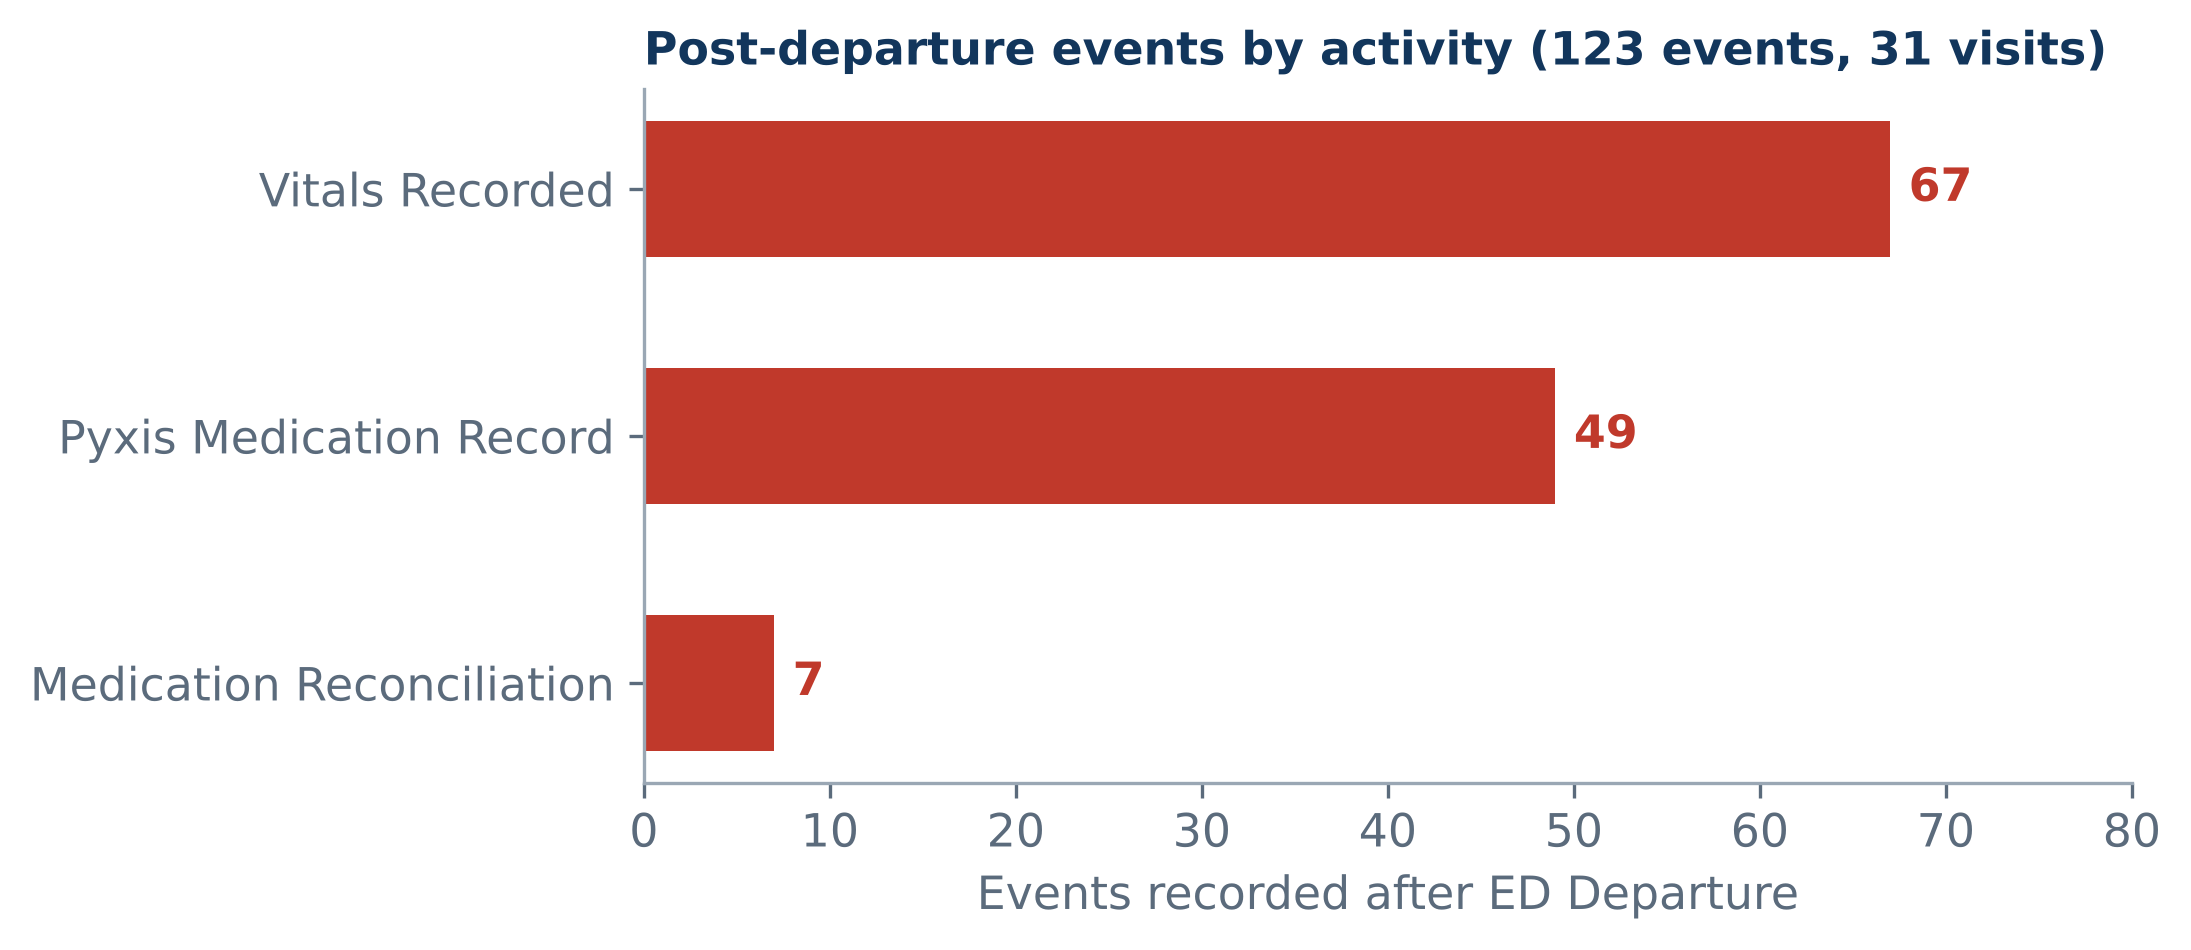
\includegraphics[width=0.72\textwidth]{images/fig_post_departure.png}
\caption{Events recorded after ED Departure, by activity.}
\end{figure}

\subsection{Limitations}
\begin{itemize}
  \item All time differences are gaps between recorded events, not confirmed clinical waiting times.
  \item Records sharing a timestamp have no provable order.
  \item Pyxis records do not prove that a medication was given.
  \item Triage and diagnosis are not in the source data.
  \item The extract is small (222 visits) and de-identified; no bottleneck, delay or clinical outcome can be concluded from it.
\end{itemize}

\begin{figure}[H]
\centering
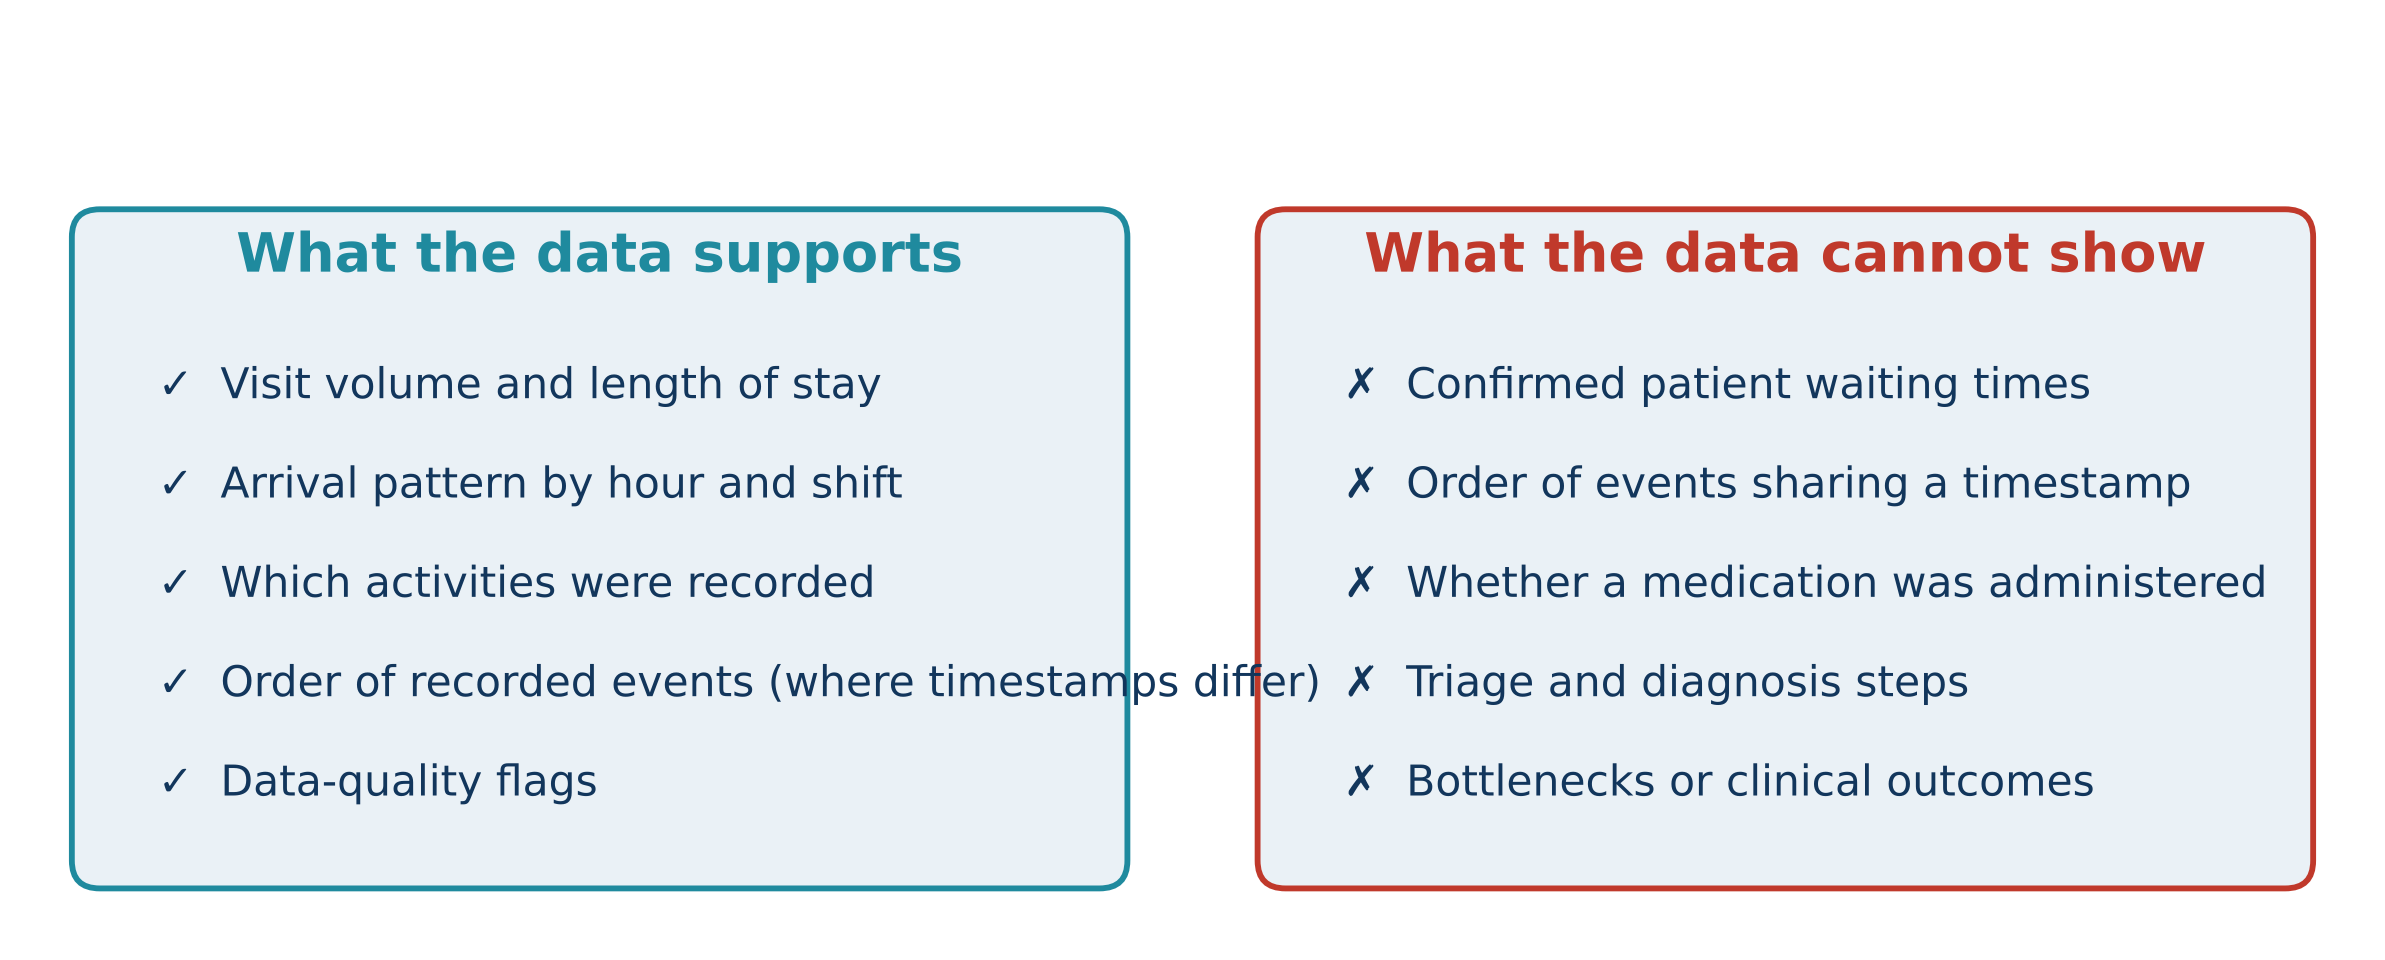
\includegraphics[width=\textwidth]{images/fig_supports_vs_limits.png}
\caption{Summary of what the extract supports and what it cannot show.}
\end{figure}

% =====================================================================
\section{Discussion and Recommendations}
The dashboard shows how the available records are distributed and where the data itself is uncertain. It does not identify clinical bottlenecks. To answer the original question about ED wait times, the following would be needed:

\begin{enumerate}[label=\textcolor{teal}{\bfseries\arabic*.}]
  \item Timestamps for Triage, provider assessment, imaging and the disposition decision, so that true waiting times can be measured.
  \item Clarification of what records stamped after ED Departure represent in the source system.
  \item An expected (mandated) workflow agreed with hospital stakeholders, so that conformance checking has a defined reference.
  \item A larger extract, so that variants and shift effects can be tested.
\end{enumerate}

% =====================================================================
\section{Conclusion and Future Work}
The team built a pipeline from an event log to a four-page Power BI dashboard covering volume, recorded activity flow, recorded event gaps and data quality. The results are descriptive and are clearly separated from claims the data cannot support. Future work includes conformance checking against an agreed workflow, richer event data, and a published version of the dashboard.

% =====================================================================
\section{Use of AI Assistance}
An AI assistant was used for planning, drafting, explanations and help with Power BI formulas and layout. All outputs were reviewed, tested against the data and understood by the author.

% =====================================================================
\appendix
\section{Appendix}
\subsection{Main DAX measures}
\begin{lstlisting}[style=dax]
Total Visits = DISTINCTCOUNT(visit_summary[Case_ID])

Median ED Stay (h) =
    DIVIDE(MEDIAN(visit_summary[LOS_Minutes]), 60)

90th Percentile Stay (h) =
    DIVIDE(PERCENTILE.INC(visit_summary[LOS_Minutes], 0.9), 60)

% Visits Over 8h =
    DIVIDE(
        CALCULATE(COUNTROWS(visit_summary), visit_summary[LOS_Minutes] > 480),
        [Total Visits]
    )

Post-Departure Events = COUNTROWS(post_departure_events)
\end{lstlisting}

\subsection{Project repository}
The project code and documentation are kept in the team repository \textbf{CareFlowG05} on GitHub.

\subsection{References}
\begin{enumerate}[label=\textcolor{teal}{[\arabic*]}]
  \item Infotact Solutions, \emph{Project Document: Advanced Data Analytics (Vol.\ II), Project 3, CareFlow}.
  \item W.\,M.\,P.\ van der Aalst, \emph{Process Mining: Data Science in Action}, 2nd ed., Springer, 2016.
  \item A.\ Berti, S.\,J.\ van Zelst and W.\,M.\,P.\ van der Aalst, ``Process Mining for Python (PM4Py): Bridging the Gap Between Process- and Data Science,'' \emph{ICPM Demo Track}, 2019.
  \item Microsoft, \emph{Power BI Desktop and DAX documentation}, Microsoft Learn.
\end{enumerate}

\end{document}
